% Options for packages loaded elsewhere
\PassOptionsToPackage{unicode}{hyperref}
\PassOptionsToPackage{hyphens}{url}
\PassOptionsToPackage{dvipsnames,svgnames,x11names}{xcolor}
%
\documentclass[
  letterpaper,
  DIV=11,
  numbers=noendperiod]{scrartcl}

\usepackage{amsmath,amssymb}
\usepackage{lmodern}
\usepackage{iftex}
\ifPDFTeX
  \usepackage[T1]{fontenc}
  \usepackage[utf8]{inputenc}
  \usepackage{textcomp} % provide euro and other symbols
\else % if luatex or xetex
  \usepackage{unicode-math}
  \defaultfontfeatures{Scale=MatchLowercase}
  \defaultfontfeatures[\rmfamily]{Ligatures=TeX,Scale=1}
\fi
% Use upquote if available, for straight quotes in verbatim environments
\IfFileExists{upquote.sty}{\usepackage{upquote}}{}
\IfFileExists{microtype.sty}{% use microtype if available
  \usepackage[]{microtype}
  \UseMicrotypeSet[protrusion]{basicmath} % disable protrusion for tt fonts
}{}
\makeatletter
\@ifundefined{KOMAClassName}{% if non-KOMA class
  \IfFileExists{parskip.sty}{%
    \usepackage{parskip}
  }{% else
    \setlength{\parindent}{0pt}
    \setlength{\parskip}{6pt plus 2pt minus 1pt}}
}{% if KOMA class
  \KOMAoptions{parskip=half}}
\makeatother
\usepackage{xcolor}
\setlength{\emergencystretch}{3em} % prevent overfull lines
\setcounter{secnumdepth}{-\maxdimen} % remove section numbering
% Make \paragraph and \subparagraph free-standing
\ifx\paragraph\undefined\else
  \let\oldparagraph\paragraph
  \renewcommand{\paragraph}[1]{\oldparagraph{#1}\mbox{}}
\fi
\ifx\subparagraph\undefined\else
  \let\oldsubparagraph\subparagraph
  \renewcommand{\subparagraph}[1]{\oldsubparagraph{#1}\mbox{}}
\fi

\usepackage{color}
\usepackage{fancyvrb}
\newcommand{\VerbBar}{|}
\newcommand{\VERB}{\Verb[commandchars=\\\{\}]}
\DefineVerbatimEnvironment{Highlighting}{Verbatim}{commandchars=\\\{\}}
% Add ',fontsize=\small' for more characters per line
\usepackage{framed}
\definecolor{shadecolor}{RGB}{241,243,245}
\newenvironment{Shaded}{\begin{snugshade}}{\end{snugshade}}
\newcommand{\AlertTok}[1]{\textcolor[rgb]{0.68,0.00,0.00}{#1}}
\newcommand{\AnnotationTok}[1]{\textcolor[rgb]{0.37,0.37,0.37}{#1}}
\newcommand{\AttributeTok}[1]{\textcolor[rgb]{0.40,0.45,0.13}{#1}}
\newcommand{\BaseNTok}[1]{\textcolor[rgb]{0.68,0.00,0.00}{#1}}
\newcommand{\BuiltInTok}[1]{\textcolor[rgb]{0.00,0.23,0.31}{#1}}
\newcommand{\CharTok}[1]{\textcolor[rgb]{0.13,0.47,0.30}{#1}}
\newcommand{\CommentTok}[1]{\textcolor[rgb]{0.37,0.37,0.37}{#1}}
\newcommand{\CommentVarTok}[1]{\textcolor[rgb]{0.37,0.37,0.37}{\textit{#1}}}
\newcommand{\ConstantTok}[1]{\textcolor[rgb]{0.56,0.35,0.01}{#1}}
\newcommand{\ControlFlowTok}[1]{\textcolor[rgb]{0.00,0.23,0.31}{#1}}
\newcommand{\DataTypeTok}[1]{\textcolor[rgb]{0.68,0.00,0.00}{#1}}
\newcommand{\DecValTok}[1]{\textcolor[rgb]{0.68,0.00,0.00}{#1}}
\newcommand{\DocumentationTok}[1]{\textcolor[rgb]{0.37,0.37,0.37}{\textit{#1}}}
\newcommand{\ErrorTok}[1]{\textcolor[rgb]{0.68,0.00,0.00}{#1}}
\newcommand{\ExtensionTok}[1]{\textcolor[rgb]{0.00,0.23,0.31}{#1}}
\newcommand{\FloatTok}[1]{\textcolor[rgb]{0.68,0.00,0.00}{#1}}
\newcommand{\FunctionTok}[1]{\textcolor[rgb]{0.28,0.35,0.67}{#1}}
\newcommand{\ImportTok}[1]{\textcolor[rgb]{0.00,0.46,0.62}{#1}}
\newcommand{\InformationTok}[1]{\textcolor[rgb]{0.37,0.37,0.37}{#1}}
\newcommand{\KeywordTok}[1]{\textcolor[rgb]{0.00,0.23,0.31}{#1}}
\newcommand{\NormalTok}[1]{\textcolor[rgb]{0.00,0.23,0.31}{#1}}
\newcommand{\OperatorTok}[1]{\textcolor[rgb]{0.37,0.37,0.37}{#1}}
\newcommand{\OtherTok}[1]{\textcolor[rgb]{0.00,0.23,0.31}{#1}}
\newcommand{\PreprocessorTok}[1]{\textcolor[rgb]{0.68,0.00,0.00}{#1}}
\newcommand{\RegionMarkerTok}[1]{\textcolor[rgb]{0.00,0.23,0.31}{#1}}
\newcommand{\SpecialCharTok}[1]{\textcolor[rgb]{0.37,0.37,0.37}{#1}}
\newcommand{\SpecialStringTok}[1]{\textcolor[rgb]{0.13,0.47,0.30}{#1}}
\newcommand{\StringTok}[1]{\textcolor[rgb]{0.13,0.47,0.30}{#1}}
\newcommand{\VariableTok}[1]{\textcolor[rgb]{0.07,0.07,0.07}{#1}}
\newcommand{\VerbatimStringTok}[1]{\textcolor[rgb]{0.13,0.47,0.30}{#1}}
\newcommand{\WarningTok}[1]{\textcolor[rgb]{0.37,0.37,0.37}{\textit{#1}}}

\providecommand{\tightlist}{%
  \setlength{\itemsep}{0pt}\setlength{\parskip}{0pt}}\usepackage{longtable,booktabs,array}
\usepackage{calc} % for calculating minipage widths
% Correct order of tables after \paragraph or \subparagraph
\usepackage{etoolbox}
\makeatletter
\patchcmd\longtable{\par}{\if@noskipsec\mbox{}\fi\par}{}{}
\makeatother
% Allow footnotes in longtable head/foot
\IfFileExists{footnotehyper.sty}{\usepackage{footnotehyper}}{\usepackage{footnote}}
\makesavenoteenv{longtable}
\usepackage{graphicx}
\makeatletter
\def\maxwidth{\ifdim\Gin@nat@width>\linewidth\linewidth\else\Gin@nat@width\fi}
\def\maxheight{\ifdim\Gin@nat@height>\textheight\textheight\else\Gin@nat@height\fi}
\makeatother
% Scale images if necessary, so that they will not overflow the page
% margins by default, and it is still possible to overwrite the defaults
% using explicit options in \includegraphics[width, height, ...]{}
\setkeys{Gin}{width=\maxwidth,height=\maxheight,keepaspectratio}
% Set default figure placement to htbp
\makeatletter
\def\fps@figure{htbp}
\makeatother
\newlength{\cslhangindent}
\setlength{\cslhangindent}{1.5em}
\newlength{\csllabelwidth}
\setlength{\csllabelwidth}{3em}
\newlength{\cslentryspacingunit} % times entry-spacing
\setlength{\cslentryspacingunit}{\parskip}
\newenvironment{CSLReferences}[2] % #1 hanging-ident, #2 entry spacing
 {% don't indent paragraphs
  \setlength{\parindent}{0pt}
  % turn on hanging indent if param 1 is 1
  \ifodd #1
  \let\oldpar\par
  \def\par{\hangindent=\cslhangindent\oldpar}
  \fi
  % set entry spacing
  \setlength{\parskip}{#2\cslentryspacingunit}
 }%
 {}
\usepackage{calc}
\newcommand{\CSLBlock}[1]{#1\hfill\break}
\newcommand{\CSLLeftMargin}[1]{\parbox[t]{\csllabelwidth}{#1}}
\newcommand{\CSLRightInline}[1]{\parbox[t]{\linewidth - \csllabelwidth}{#1}\break}
\newcommand{\CSLIndent}[1]{\hspace{\cslhangindent}#1}

\KOMAoption{captions}{tableheading}
\makeatletter
\makeatother
\makeatletter
\makeatother
\makeatletter
\@ifpackageloaded{caption}{}{\usepackage{caption}}
\AtBeginDocument{%
\ifdefined\contentsname
  \renewcommand*\contentsname{Table of contents}
\else
  \newcommand\contentsname{Table of contents}
\fi
\ifdefined\listfigurename
  \renewcommand*\listfigurename{List of Figures}
\else
  \newcommand\listfigurename{List of Figures}
\fi
\ifdefined\listtablename
  \renewcommand*\listtablename{List of Tables}
\else
  \newcommand\listtablename{List of Tables}
\fi
\ifdefined\figurename
  \renewcommand*\figurename{Figure}
\else
  \newcommand\figurename{Figure}
\fi
\ifdefined\tablename
  \renewcommand*\tablename{Table}
\else
  \newcommand\tablename{Table}
\fi
}
\@ifpackageloaded{float}{}{\usepackage{float}}
\floatstyle{ruled}
\@ifundefined{c@chapter}{\newfloat{codelisting}{h}{lop}}{\newfloat{codelisting}{h}{lop}[chapter]}
\floatname{codelisting}{Listing}
\newcommand*\listoflistings{\listof{codelisting}{List of Listings}}
\makeatother
\makeatletter
\@ifpackageloaded{caption}{}{\usepackage{caption}}
\@ifpackageloaded{subcaption}{}{\usepackage{subcaption}}
\makeatother
\makeatletter
\@ifpackageloaded{tcolorbox}{}{\usepackage[many]{tcolorbox}}
\makeatother
\makeatletter
\@ifundefined{shadecolor}{\definecolor{shadecolor}{rgb}{.97, .97, .97}}
\makeatother
\makeatletter
\makeatother
\ifLuaTeX
  \usepackage{selnolig}  % disable illegal ligatures
\fi
\IfFileExists{bookmark.sty}{\usepackage{bookmark}}{\usepackage{hyperref}}
\IfFileExists{xurl.sty}{\usepackage{xurl}}{} % add URL line breaks if available
\urlstyle{same} % disable monospaced font for URLs
\hypersetup{
  pdftitle={Gender differences in   parental wealth transfers and   how the German tax system contributes to the gender wealth gap},
  pdfauthor={  Daria Tisch¹ \& Manuel Schechtl²     ¹Max Planck Institute for the Study of Societies   ²Stone-Center on Socio-Economic Inequality, The Graduate Center, City University of New York},
  colorlinks=true,
  linkcolor={blue},
  filecolor={Maroon},
  citecolor={Blue},
  urlcolor={Blue},
  pdfcreator={LaTeX via pandoc}}

\title{Gender differences in parental wealth transfers and how the
German tax system contributes to the gender wealth gap}
\usepackage{etoolbox}
\makeatletter
\providecommand{\subtitle}[1]{% add subtitle to \maketitle
  \apptocmd{\@title}{\par {\large #1 \par}}{}{}
}
\makeatother
\subtitle{INAUGURAL III/LIS COMPARATIVE ECONOMIC INEQUALITY CONFERENCE
February, 25th 2023}
\author{ Daria Tisch¹ \& Manuel Schechtl² ¹Max Planck Institute for the
Study of Societies ²Stone-Center on Socio-Economic Inequality, The
Graduate Center, City University of New York}
\date{}

\begin{document}
\maketitle
\ifdefined\Shaded\renewenvironment{Shaded}{\begin{tcolorbox}[interior hidden, frame hidden, sharp corners, borderline west={3pt}{0pt}{shadecolor}, boxrule=0pt, enhanced, breakable]}{\end{tcolorbox}}\fi

\hypertarget{gender-wealth-gap}{%
\subsection{Gender wealth gap}\label{gender-wealth-gap}}

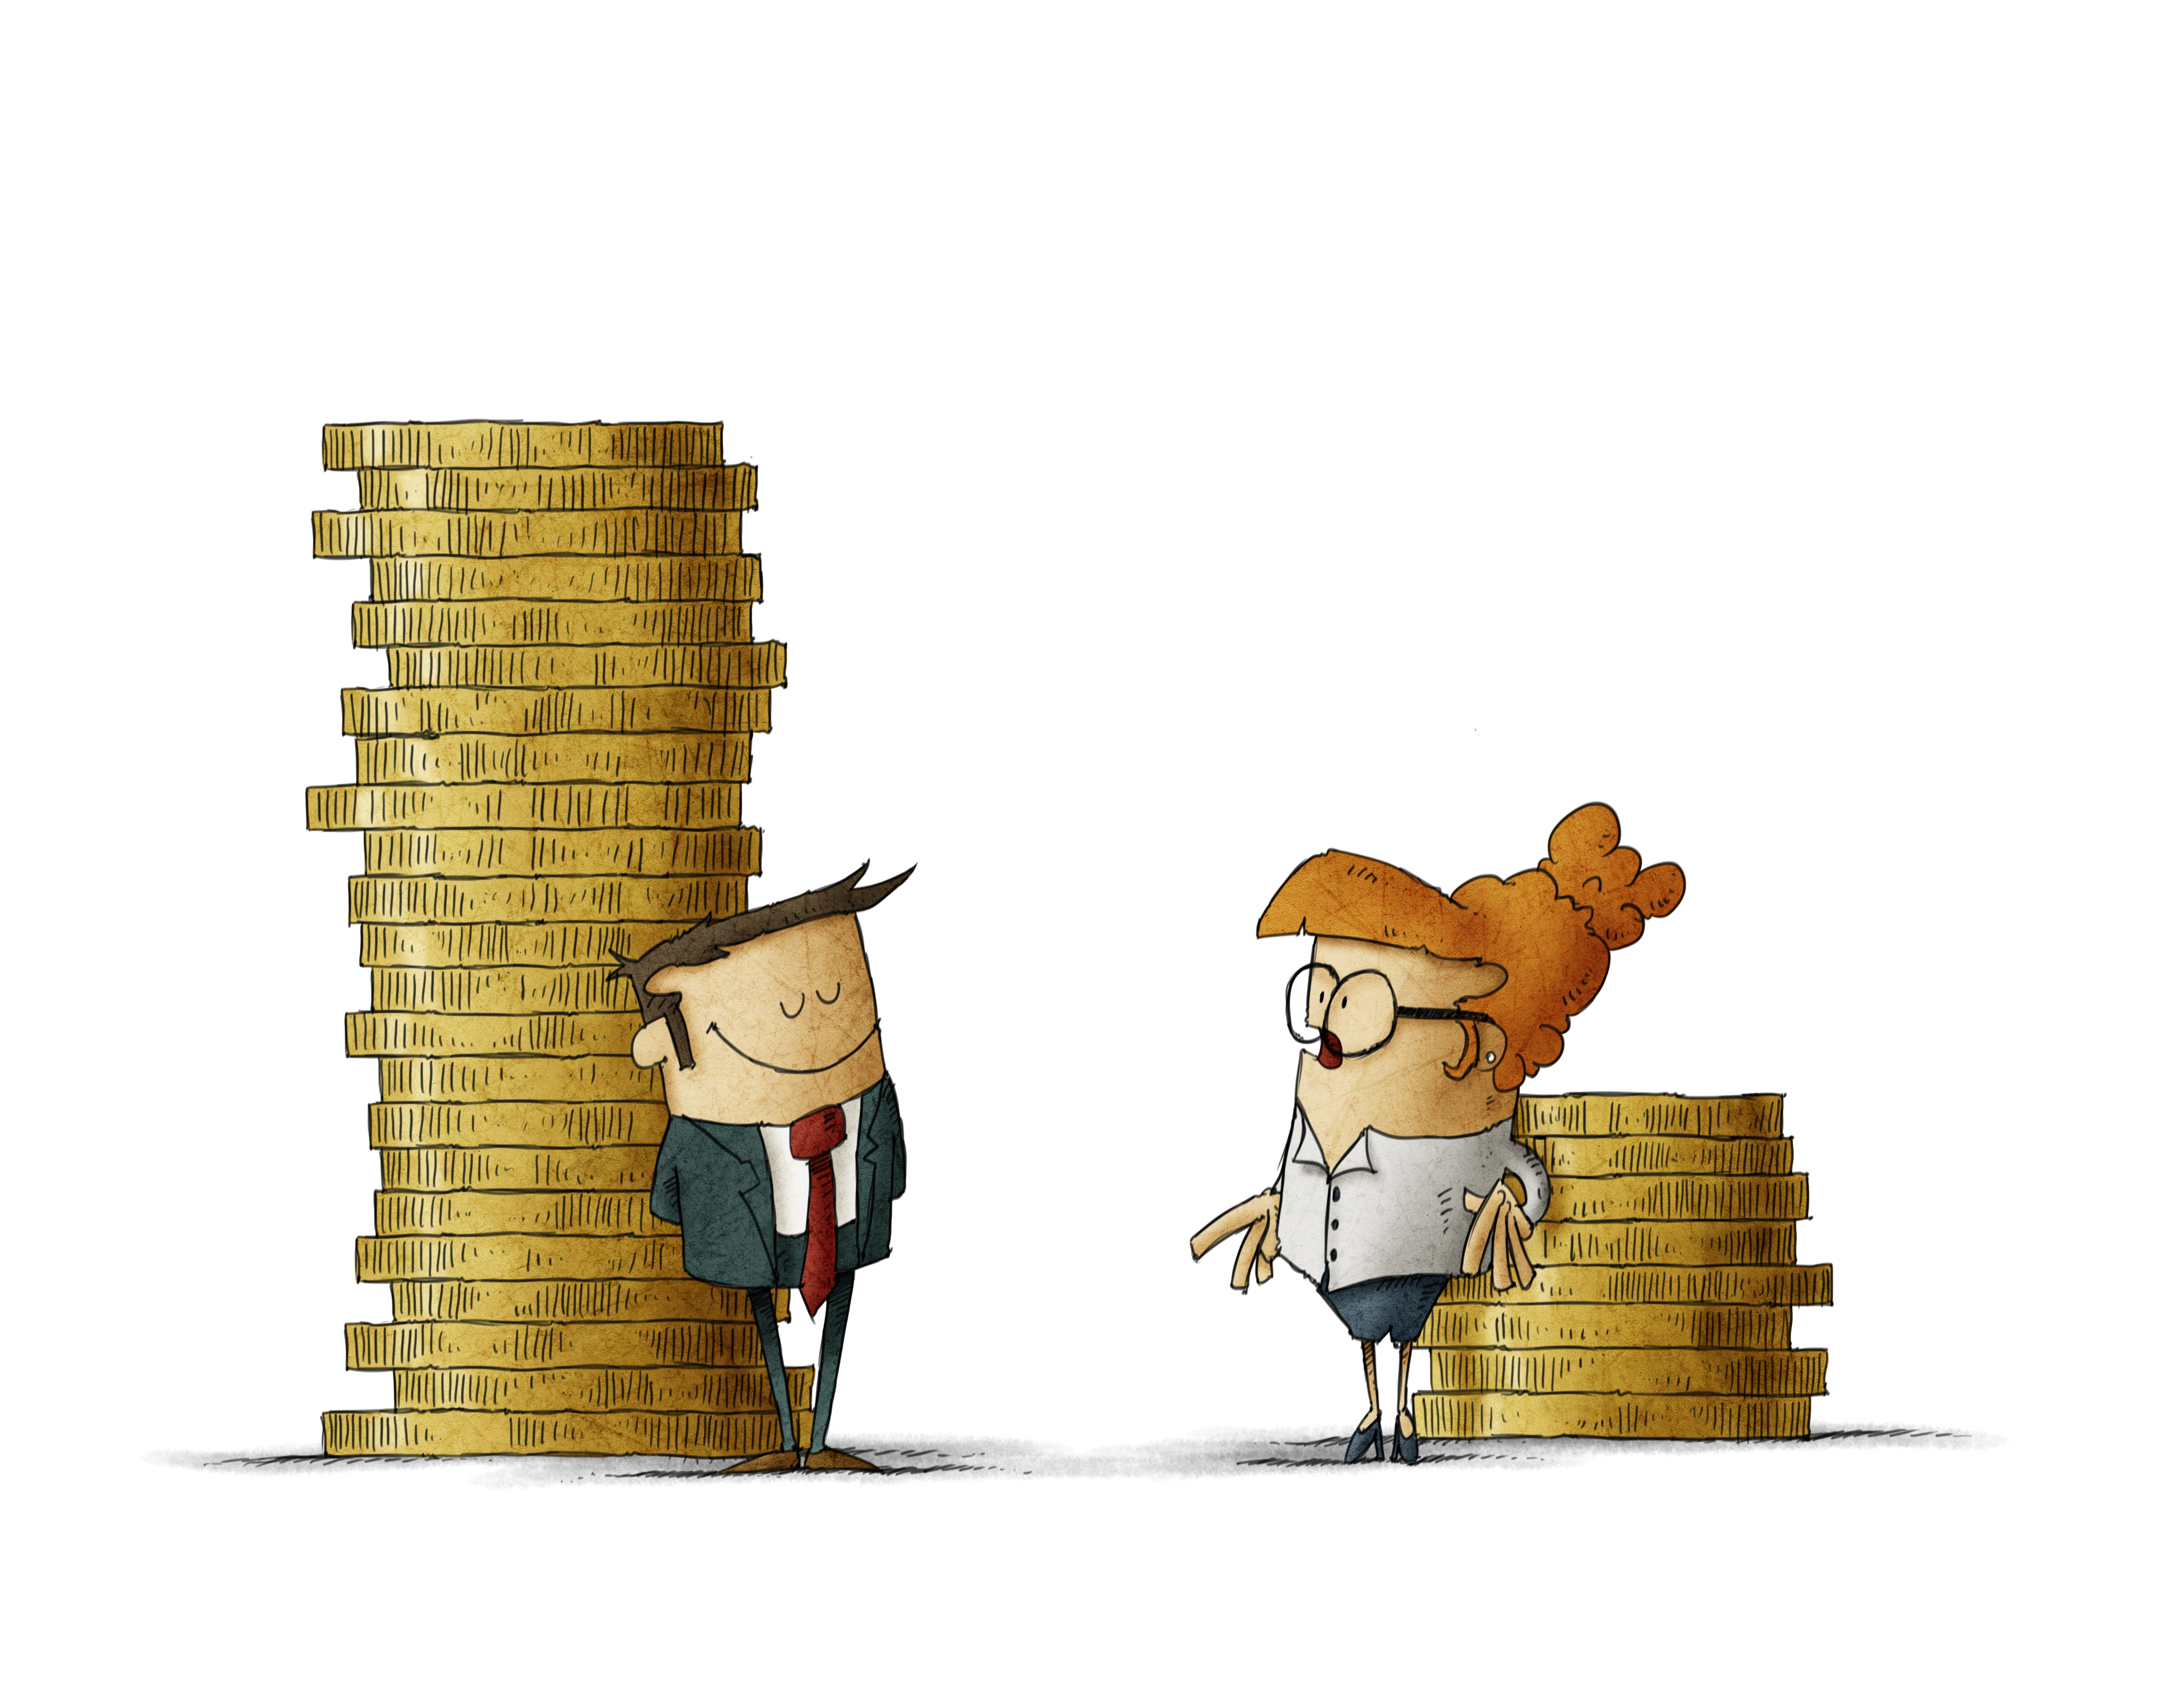
\includegraphics[width=1\textwidth,height=\textheight]{images/luecke_gekauft.jpg}

\begin{itemize}
\tightlist
\item
  Gender wealth gap well established, on average Men own more wealth
  than women in most countries around the world.
\item
  Prior research showed that differences in income and employment
  explain gender differences in wealth
\item
  But intergenerational transfers might also play a role
\item
  as does the tax system
\item
  So both intergenerational transfers and taxes have been neglected in
  the literature on the gender wealth gap. We want to change that with
  this project.
\end{itemize}

\hypertarget{motivation}{%
\subsection{Motivation}\label{motivation}}


\includegraphics[width=4.16667in,height=\textheight]{images/transfers.jpg}

\begin{itemize}
\tightlist
\item
  Share of inherited wealth in aggregate private wealth in Europe around
  50-60\% (Alvaredo, Garbinti, and Piketty 2017)
\item
  What's the role of intergenerational transfers in gender wealth
  inequality?

  \begin{itemize}
  \item
    Gender difference in age and amounts of transfers (Bessière and
    Gollac 2020)
  \item
    Hardly any gender differences in \textbf{inheritances} in Germany
    (Leopold and Schneider 2011; Vogel et al. 2021)
  \item
    Daughters more likely to receive inter vivos transfer but only until
    they are married (Loxton 2019)
  \item
    But: Prior research based on \textbf{survey data}
  \end{itemize}
\end{itemize}

Let me motviate why we should look at intergenerational transfers?

\begin{itemize}
\item
  Most personal wealth today is inherited. Share of inherited wealth in
  aggregate wealth is estimated to be around 50-60\%.
\item
  So if private wealth is so much shaped by inheritance it is only
  logical to ask how intergenerational transfers contribute to the
  gender wealth gap
\item
  Prior literature on this topic is limited. For France, Bessiere and
  Gollac show that men receive transfers at earlier ages and higher
  amounts leading to a higher accumulation potential
\item
  Hardly any gender differences are found in Germany for inheritances.
  Some for gifts.
\item
  In the US, daughters more likely to receive transfers but no
  difference in amounts. And increased likelihood only for unmarried
  daughters.
\item
  The problem of these study is that they are based on survey data which
  do not represent the upper end of the wealth distribution well.
  Because wealth is highly concentrated and power comes along with
  wealth, it is especially important to know more about gender
  differences at the top of the wealth transfer distribution.
\end{itemize}

\hypertarget{research-question-contributions}{%
\subsection{Research question \&
contributions}\label{research-question-contributions}}

\hypertarget{research-question}{%
\subsubsection{Research question}\label{research-question}}

How does the inheritance and gift tax system shape gender inequalities
in parental transfers?

\hypertarget{contributions}{%
\subsubsection{Contributions}\label{contributions}}

\begin{itemize}
\item
  Focus on the upper part of the transfer distribution
\item
  Differentiation between asset types
\item
  Role of the tax system in shaping gender wealth inequality
\end{itemize}

\begin{itemize}
\tightlist
\item
  In our study we ask: How does the inheritance and gift tax system
  shape gender inequalities in parental transfers?

  \begin{itemize}
  \item
    Are there gender differences in parental transfers (inheritances and
    gifts) in Germany?
  \item
    How does the German inheritance and gift tax system shape gender
    inequalities?
  \end{itemize}
\item
  I think we make three major contributions with this study

  \begin{enumerate}
  \def\labelenumi{\arabic{enumi}.}
  \tightlist
  \item
    We add to prior literature by looking at the top of the transfer
    distribution: Upper part important because wealth is related to
    power
  \item
    We differentiate between assets types. It is important to
    differentiate between asset types because they offer different
    accumulation potential and translate differently into power. It
    makes a difference if you inherited a house or a business
  \item
    We contribute to the questions how institutions shape wealth
    inequality by looking at the tax system. here the idea is that men
    and women benefit differently from tax exemptions because they
    receive different kind of assets
  \end{enumerate}
\end{itemize}

\hypertarget{theoretical-background}{%
\subsection{Theoretical background}\label{theoretical-background}}

\hypertarget{gender-bias-in-taxation}{%
\subsubsection{Gender bias in taxation}\label{gender-bias-in-taxation}}

\begin{itemize}
\tightlist
\item
  explicit gender bias: tax law treats men and women differently
\item
  implicit gender bias: tax law has different implications for women and
  men because of \textbf{gendered social arrangements and economic
  behavior} (Stotsky 1996)
\end{itemize}

\hypertarget{gender-differences-in-parental-transfers}{%
\subsubsection{Gender differences in parental
transfers}\label{gender-differences-in-parental-transfers}}

\begin{itemize}
\tightlist
\item
  Family as a place where wealth is produced, circulated, controlled,
  and assigned value (Bessière and Gollac 2020)
\item
  Societal beliefs in gender differences in entitlements (Lerner and
  Mikula 1994; Tisch and Gutfleisch 2022)
\item
  Daughters and sons might receive different asset types which leads to
  different tax exemptions
\end{itemize}

What is the theoretical background? We follow the literature in arguing
that the family is an important economic institution. The family is a
place where wealth is produced, circulated, controlled, and assigned
value. And the family contributes to wealth inequality via
intergenerational transfers.

But why should the family treat daughters and sons differently?

Sons and daughters might receive different amounts of transfers,
different assets types or they might be more or less likely to receive a
transfer at all. This could be because of gendered norms or because of
gender differences in characteristics which trigger transfers.

\begin{itemize}
\item
  There might be societal beliefs in gendered entitlements to transfers.
  In a recent study Tamara Gutfleisch and I find first evidence for
  gendered transfer principles although most individuals endorse
  equality.
\item
  But even if their are no gendered beliefs, gender difference might
  arise. Parents might be in a conflict between pursing the principle of
  equality but also other principles like the exchange or
  need/altruistic principle. The parents might also want to keep the
  fortunes together. To this end it might make sense to transfer wealth
  unequally between children. So it might be the case that there are
  gender differences in the characteristics which trigger these
  principles. For example that women are more likely to be in need of
  financial help and therefore receive more transfers.
\item
  And last, gender inequality in transfers might also be the product of
  the tax system. It could be that men benefit more from tax exemptions
  than women because they receive assets which benefit from larger tax
  exemptions.
\end{itemize}

\hypertarget{country-context-german-gift-and-inheritance-tax-law}{%
\subsection{\texorpdfstring{Country context: German gift and inheritance
(tax)
law}{Country context:   German gift and inheritance (tax) law}}\label{country-context-german-gift-and-inheritance-tax-law}}

\begin{itemize}
\tightlist
\item
  Inheritances

  \begin{itemize}
  \tightlist
  \item
    statutory inheritance quota or last will (predefined inheritance +
    quota)
  \item
    restricted testamentary freedom → disinheritance possible but
    statutory share: minimum inheritance of close relatives is half the
    amount they would have received in absence of a last will
  \end{itemize}
\item
  Gifts: amount of the gift and the recipient can be freely determined
\item
  Inheritance tax (not an estate tax)

  \begin{itemize}
  \tightlist
  \item
    personal tax exemption (applies to the taxable person): e.g.,
    400,000 EUR / 10 years for parental transfer
  \item
    factual tax exemption (applies to the taxable object): business,
    forest, furniture, family home etc.
  \end{itemize}
\end{itemize}

Before you die you have basically two options: writing a last will or
not

\begin{itemize}
\item
  if you don't write a last will the statutory inheritance quota will be
  in place with no gender discrimination
\item
  or you write a last will and can specify the quota or also predefine
  inheritance. eg you can say that your son should receive the house
\item
  The testamentary freedom is restricted in Germany. You can disinherit
  a child but then this child can claim their statutory share from the
  legal heir. This share is half of the amount they would receive in the
  absence of a will
\item
  There are no regulations regarding gift. Thus, the amount and
  recipient of gifts can be freely chosen
\item
  What about taxes?

  \begin{itemize}
  \item
    inheritance tax not an estate tax like in the US
  \item
    gifts and inheritances are treated equally
  \item
    personal tax exemptions which apply to the taxable person: eg
    400,000 Euro every 10 years for each parent
  \item
    factual exemptions which apply to the taxable object: business,
    forest land, furniture, family home
  \end{itemize}
\end{itemize}

\hypertarget{data}{%
\subsection{Data}\label{data}}

\includegraphics[width=4.16667in,height=\textheight]{images/steuererkl.jpg}

\begin{itemize}
\tightlist
\item
  German inheritance and gift tax data 2007-2020
\item
  Highly sensitive data → restricted access
\item
  Cover bequests and gifts for which a tax claim was requested
\item
  Advantage: Entire population of tax relevant transfers
\item
  Coverage: 30\% of all bequests, accounting for 73\% of all transferred
  wealth above 10,000 EUR in 2010 (Bach et al. 2014)
\end{itemize}

\hypertarget{methods}{%
\subsection{Methods}\label{methods}}

\begin{itemize}
\item
  Descriptive analyses
\item
  OLS regressions

  \begin{itemize}
  \item
    Dependent variables: Effective inheritance / gift tax rate
  \item
    Predictor variables

    \begin{itemize}
    \tightlist
    \item
      gender (receiver and donor)
    \item
      asset type (as dummy variables)
    \item
      age (receiver and donor)
    \item
      east/west Germany
    \item
      year
    \end{itemize}
  \end{itemize}
\end{itemize}

Our methods are very straightforward, we look at descriptive tables and
graphs. And to explain the gender gap we run OLS regressions.

\begin{itemize}
\item
  dependent variable are the amount of gifts and inheritance. Due to the
  skewdness of the data, we transform the data by a percentile rank
  transformation (for each year separately)
\item
  second group of dependent variables are the effective tax rate.
  Inheritance and gift
\item
  our predictor variables are: gender, asset type, age, east/west, year
\end{itemize}

\hypertarget{section}{%
\subsection{}\label{section}}

{Gendered transfer behavior: Gender inequality in gifts but not
inheritances?}

\hypertarget{gender-ratio-in-transfers-over-time}{%
\subsection{Gender ratio in transfers over
time}\label{gender-ratio-in-transfers-over-time}}

\begin{Shaded}
\begin{Highlighting}[]
\NormalTok{over\_time\_ratio}
\end{Highlighting}
\end{Shaded}

\begin{figure}[H]

{\centering \includegraphics{dgs_files/figure-pdf/unnamed-chunk-2-1.pdf}

}

\end{figure}

\begin{itemize}
\tightlist
\item
  Because we are interested in the gender differences we now examine the
  gender ratios.
\item
  What you see here is the gender ratio calculated as male/female for
  different quantiles.
\item
  The red line at the value of 1 represents equal transfers. If the
  value is above 1 men receive more, if the value is below 1 men receive
  less than women.
\item
  the black dots represents inheritances and the gray dots gifts.
\item
  and the straight lines indicate the average across all years
\item
  Let's look at the median. We see that the amount of transfers does not
  differ at the median between women and men for inheritances. But it
  does for gifts. On average, the median gift received by men is 10\%
  higher than the one of women.
\item
  gender differences are more pronounced in the 90th quantile
\item
  But it is problematic to only look at the amount of transfers. We
  should also look at the ratio of the number of transfers. And here we
  see that men receive 10\% more inheritances than women. But men
  receive over 40\% more gifts than women.
\end{itemize}

\hypertarget{gender-ratio-in-the-number-of-transfers-including-specific-components-by-deciles}{%
\subsection{Gender ratio in the number of transfers including specific
components by
deciles}\label{gender-ratio-in-the-number-of-transfers-including-specific-components-by-deciles}}

\begin{Shaded}
\begin{Highlighting}[]
\NormalTok{gcomp\_dec\_erb\_gift}
\end{Highlighting}
\end{Shaded}

\begin{figure}[H]

{\centering \includegraphics{dgs_files/figure-pdf/unnamed-chunk-3-1.pdf}

}

\end{figure}

\begin{itemize}
\tightlist
\item
  So what about the type of assets. Do women and men also differ in the
  type of assets they receive. It is important to examine if women and
  men receive different kind of assets because different assets have
  different accumulation potential
\item
  Here we only look at the number of gifts! Again we calculate the ratio
  as men/women
\item
  In this graph we see the gender ratio in the number of gifts which
  include the respective asset type.
\item
  on the x axis we have now deciles and not year. So the dots represent
  the average across all deciles
\item
  The upper left graph shows that men receive two times as many gifts
  including business assets as women
\item
  For land, the ratio is even more extreme especially at the top of the
  distribution
\item
  the smallest gender differences in the amount of gifts are estates and
  others
\end{itemize}

\hypertarget{section-1}{%
\subsection{}\label{section-1}}

{Let's look at how the tax system shapes gender inequality.}

We now turn to the second research question. - To understand how the tax
systems affects gender inequality, we calculate the effective tax rate
and compare women and men 1. We examine the absolute effective tax rate
of women and men across the transfer distribution 2. We examine the
absolute effective tax rate by the gender of the donor 3. And we then
look at the relative effective tax rates. So we examine how much more
women have to pay in taxes compared to men 4. Last, we try to explain
the gender tax gap with an OLS regression. We focus here on the asset
type and gender of the donor

\hypertarget{effective-inheritance-tax-rate-by-gender-of-receiver-2007-2020}{%
\subsection{Effective inheritance tax rate by gender of receiver
(2007-2020)}\label{effective-inheritance-tax-rate-by-gender-of-receiver-2007-2020}}

dag
\includegraphics[width=0.85\textwidth,height=\textheight]{images/output4b_gepr.png}

This graph shows the effective tax rate on the y axis and the percentile
distribution of parental inheritance on the x axis. The percentile
distribution is calculated jointly for men and women.

\begin{itemize}
\tightlist
\item
  We do not find big gender differences in the effective inheritance tax
  rate. Only at the top of the wealth distribution, daughter have to pay
  more taxes than sons.
\end{itemize}

\hypertarget{effective-gift-tax-rate-by-gender-of-receiver-2007-2020}{%
\subsection{Effective gift tax rate by gender of receiver
(2007-2020)}\label{effective-gift-tax-rate-by-gender-of-receiver-2007-2020}}

\includegraphics[width=0.85\textwidth,height=\textheight]{images/output4d_gepr.png}

But that looks different for gifts.

\begin{itemize}
\item
  So you see here the same graph but on the x axis the parental gift
  distribution.
\item
  Women pay on average 1 percentage point more gift taxes than men.
\item
  Gift tax indirectly discriminates women because men benefit from tax
  exemptions.
\end{itemize}

\hypertarget{gender-gap-of-effective-tax-rate-over-time}{%
\subsection{Gender gap of effective tax rate over
time}\label{gender-gap-of-effective-tax-rate-over-time}}

\begin{Shaded}
\begin{Highlighting}[]
\NormalTok{over\_time\_ratio\_taxrate2}
\end{Highlighting}
\end{Shaded}

\begin{verbatim}
Warning: Removed 11 rows containing missing values (`geom_point()`).
\end{verbatim}

\begin{verbatim}
Warning: Removed 1 rows containing missing values (`geom_hline()`).
\end{verbatim}

\begin{figure}[H]

{\centering \includegraphics{dgs_files/figure-pdf/unnamed-chunk-4-1.pdf}

}

\end{figure}

\begin{itemize}
\tightlist
\item
  Let us know look at the gender ratio in the effective tax rate over
  time.
\item
  On the y axis you see the gender ratio which is calculated as tax of
  men/ tax of women
\item
  values below 1 indicate that women pay more taxes. Values above 1
  indicate that men pay more taxes
\item
  Let's look at the mean, the upper left panel
\item
  Men pay about 20\% less taxes on gifts than women on average but Men
  pay only 1-3\% less taxes on inheritance than women on average
\item
  Let's move to the median in the upper right panel. Here, At the median
  a gender tax gap is visible also for inheritance and it amounts to
  about 18\%.
\item
  Interestingly we see that 50\% of the receiver of gifts payed no tax
  at all indicated by missing dots in the upper right panel.
\end{itemize}

\hypertarget{regression-effective-gift-tax-2007-2020}{%
\subsection{Regression: effective gift tax
(2007-2020)}\label{regression-effective-gift-tax-2007-2020}}

\begin{Shaded}
\begin{Highlighting}[]
\NormalTok{t\_reg\_gifts\_tax }
\end{Highlighting}
\end{Shaded}

\begin{longtable}[]{@{}lllll@{}}
\toprule()
& M1 (b) & M1 (se) & M2 (b) & M2 (se) \\
\midrule()
\endhead
Receiver female & 0.549*** & 0.02 & 0.480** & 0.17 \\
Gifts, percentile & 0.0113*** & 0.00 & 0.0287*** & 0.00 \\
Business (indicator) & & & -2.138*** & 0.05 \\
Business (indicator) * Receiver female & & & -0.448*** & 0.08 \\
Land (indicator) & & & -1.260*** & 0.05 \\
Land (indicator) * Receiver female & & & 0.0853 & 0.09 \\
Other wealth (indicator) & & & 1.235*** & 0.04 \\
Other wealth (indicator) * Receiver female & & & 0.127 & 0.08 \\
Estate (indicator) & & & -1.147*** & 0.04 \\
Estate (indicator) * Receiver female & & & -0.752*** & 0.08 \\
Donor female & & & 0.0220 & 0.03 \\
Donor female * Receiver female & & & -0.338*** & 0.05 \\
Age (receiver) & & & 0.0656*** & 0.00 \\
Age (receiver) * Receiver female & & & -0.0102*** & 0.00 \\
Age (donor) & & & 0.00333** & 0.00 \\
Age (donor) * Receiver female & & & 0.00848*** & 0.00 \\
West & & & 0.659*** & 0.05 \\
West * Receiver female & & & -0.188* & 0.08 \\
& & & 0.00719*** & 0.00 \\
Intercept & 2.812*** & 0.05 & -0.623*** & 0.12 \\
N & 271087 & & 255949 & \\
R² & 0.02 & & 0.11 & \\
Gender Gap & 0.549 & & 0.348 & \\
p value (Gender Gap) & 0.00 & & 0.00 & \\
\bottomrule()
\end{longtable}

\begin{itemize}
\item
  Last, we estimated regressions with the effective tax as the dependent
  variable.
\item
  For gifts we find that daughters pay on average 0.5 percentage points
  more than sons. Raw gift tax gap.
\item
  The wealth components explain part of this gender gift tax gap. The
  gender tax gap decreases if business wealth is included in the
  transfer.
\item
  The gender tax gap decreases also if estate wealth is included
\item
  Thus, the regression shows that men and women benefit differently from
  the tax exemption leading to the gender tax gap.
\item
  interestingly, the tax gap is also smaller if the donor is female.
\item
  Let's just look shortly at the other coefficients: if you receive
  business you pay less tax. This basically refelects the tax
  exemptions.
\end{itemize}

\hypertarget{regression-effective-inheritance-tax}{%
\subsection{Regression: effective inheritance
tax}\label{regression-effective-inheritance-tax}}

\begin{Shaded}
\begin{Highlighting}[]
\NormalTok{t\_reg\_inheritance\_tax}
\end{Highlighting}
\end{Shaded}

\begin{longtable}[]{@{}lllll@{}}
\toprule()
& M1 (b) & M1 (se) & M2 (b) & M2 (se) \\
\midrule()
\endhead
Receiver female & 0.0804*** & 0.02 & -0.0708 & 0.18 \\
Inheritance, percentile & 0.119*** & 0.00 & 0.119*** & 0.00 \\
Business (indicator) & & & -0.558*** & 0.04 \\
Business (indicator) * Receiver female & & & 0.463*** & 0.06 \\
Land (indicator) & & & -0.311*** & 0.04 \\
Land (indicator) * Receiver female & & & 0.223*** & 0.05 \\
Other wealth (indicator) & & & 0.822*** & 0.05 \\
Other wealth (indicator) * Receiver female & & & -0.378*** & 0.08 \\
Estate (indicator) & & & -1.386*** & 0.03 \\
Estate (indicator) * Receiver female & & & -0.0885 & 0.05 \\
Donor female & & & -0.114*** & 0.03 \\
Donor female * Receiver female & & & -0.0548 & 0.04 \\
Age (receiver) & & & -0.0115*** & 0.00 \\
Age (receiver) * Receiver female & & & -0.00309 & 0.00 \\
Age (donor) & & & 0.0276*** & 0.00 \\
Age (donor) * Receiver female & & & 0.00216 & 0.00 \\
West & & & 0.117 & 0.06 \\
West * Receiver female & & & 0.0355 & 0.09 \\
& & & 0.00849*** & 0.00 \\
Intercept & -0.883*** & 0.04 & -2.210*** & 0.13 \\
N & 239947 & & 229733 & \\
R² & 0.38 & & 0.39 & \\
Gender Gap & 0.080 & & 0.070 & \\
p value (Gender Gap) & 0.00 & & 0.00 & \\
\bottomrule()
\end{longtable}

And last, for the effective tax paid on inheritances we find a very
small gender tax gap of only 0.1 percentage points. It is still
significant.

And again the coefficients reflect the tax exemptions of the inheritance
tax law.

\hypertarget{conclusion}{%
\subsection{Conclusion}\label{conclusion}}

\hypertarget{gendered-parental-transfers}{%
\subsubsection{Gendered parental
transfers}\label{gendered-parental-transfers}}

\begin{itemize}
\tightlist
\item
  Gender differences in total number of inheritances and gift
\item
  More pronounced for gifts
\item
  More pronounced for transfers including business and land wealth
\end{itemize}

\hypertarget{implicit-gender-bias-in-inheritance-and-gift-taxation}{%
\subsubsection{Implicit gender bias in inheritance and gift
taxation}\label{implicit-gender-bias-in-inheritance-and-gift-taxation}}

\begin{itemize}
\tightlist
\item
  Men's effective inheritance tax rate 2\% lower than women's
\item
  Men's effective gift tax rate 18\% lower than women's
\end{itemize}

→ Tax system with generous exemptions amplifies gender inequality

{Contact:} {tisch@mpifg.de} \textbar{}
{\url{https://dariatisch.github.io/}}

\begin{itemize}
\tightlist
\item
  To conclude, we identified varies gender gaps.
\item
  the number of tax relevant inheritances are 8\% higher for men
  compared to women
\item
  the number of tax relevant gifts are even 43\% higher for men compared
  to women
\item
  the gender gap in the amounts of inheritances are smalll
\item
  At the 90th quantile gifts received by men are 20\% higher than gifts
  received by women.
\item
  We showed that gender differences are more pronounces for gifts
  compared to inheritances. This raises the question if the egalitarian
  inheritance law reduces gender wealth inequality by either spread
  egalitarian norms or because many dont specify a last will.
\item
  We also showed that women and men receive differert types of assets
  types and that explains party the gender transfer gap in amounts. Both
  our analyses indicates also that especially male donor seem to be
  responsible for the gender transfer gap by favoring sons
\item
  Last, we identified a gender inheritance tax gap of 0.97 and a gender
  gift gap of 0.79. Indicating that women pay on average about 20\%
  higher taxes compared to men. This indicates that the tax system with
  its generous exemptions amplifies gender inequality.
\end{itemize}

\hypertarget{references}{%
\subsection{References}\label{references}}

\hypertarget{refs}{}
\begin{CSLReferences}{1}{0}
\leavevmode\vadjust pre{\hypertarget{ref-alvaredo2017}{}}%
Alvaredo, Facundo, Bertrand Garbinti, and Thomas Piketty. 2017. {``On
the Share of Inheritance in Aggregate Wealth: Europe and the USA,
1900{\textendash}2010.''} \emph{Economica} 84 (334): 239--60.
\url{https://doi.org/10.1111/ecca.12233}.

\leavevmode\vadjust pre{\hypertarget{ref-bach2014}{}}%
Bach, Stefan, Henriette Houben, Ralf Maiterth, and Richard Ochmann.
2014. {``Aufkommens-Und Verteilungswirkungen von Reformalternativen Für
Die Erbschaft-Und Schenkungsteuer. Endbericht: Forschungsprojekt Im
Auftrag Der Bundestagsfraktion Bündnis 90/Die Grünen.''}
\emph{Politikberatung Kompakt}.

\leavevmode\vadjust pre{\hypertarget{ref-bessiuxe8re2020}{}}%
Bessière, Céline, and Sibylle Gollac. 2020. \emph{Genre Du Capital :
Comment La Famille Reproduit Les Inégalités}. Paris: Découverte.

\leavevmode\vadjust pre{\hypertarget{ref-leopold2011}{}}%
Leopold, Thomas, and Thorsten Schneider. 2011. {``Intergenerationale
Vermögenstransfers Und Soziale Ungleichheit.''} In, 49--72. Springer.

\leavevmode\vadjust pre{\hypertarget{ref-lerner1994}{}}%
Lerner, Melvin J., and Gerold Mikula. 1994. \emph{Entitlement and the
Affectional Bond. Justice in Close Relationships}. Critical I. Boston,
MA: Springer.

\leavevmode\vadjust pre{\hypertarget{ref-loxton2019}{}}%
Loxton, Abigail. 2019. {``Gender Differences in Inter Vivos
Transfers.''} \emph{CAEPR Working Papers} 2: 1--24.
\url{https://doi.org/10.2139/ssrn.3342730}.

\leavevmode\vadjust pre{\hypertarget{ref-stotsky1996}{}}%
Stotsky, Ms Janet Gale. 1996. \emph{Gender Bias in Tax Systems}.
International Monetary Fund.

\leavevmode\vadjust pre{\hypertarget{ref-tisch2022}{}}%
Tisch, Daria, and Tamara Gutfleisch. 2022. {``Unequal but Just ?
Experimental Evidence on Distributive Justice Principles in Parental
Inter Vivos Transfers.''} \emph{Socio-Economic Review}.

\leavevmode\vadjust pre{\hypertarget{ref-vogel2021a}{}}%
Vogel, Claudia, H. Künemund, K. Baresel, H. Eulitz, U. Fachinger, M. M.
Grabka, C. Halbmeier, and A. Lozano Alcántara. 2021. {``Gleiche
Erbchancen Für Frauen Und Männer? Zur Geschlechtsspezifschen Bedeutung
von Erbschaften Für Die Alterssicherung.''} \emph{Deutsche
Rentenversicherung} 3: 236--51.

\end{CSLReferences}



\end{document}
